\documentclass{article}
\usepackage{tikz}
\usetikzlibrary{arrows.meta}

\begin{document}

\begin{figure}[h]
    \centering
    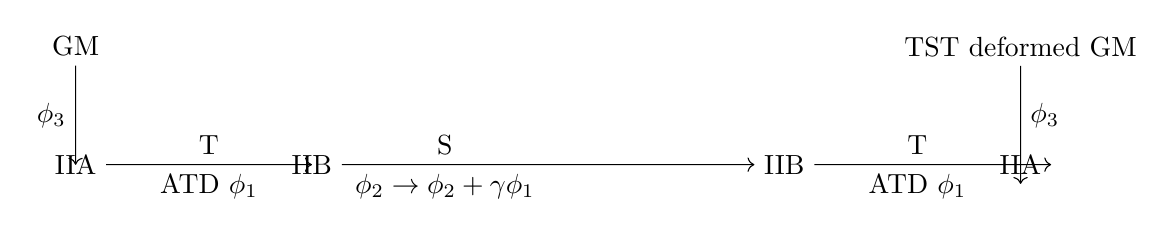
\begin{tikzpicture}[scale=1.5]
        % Draw the GM node
        \node (GM) at (-2, 0) {GM};
        
        % Draw the IIA node
        \node (IIA) at (-2, -1) {IIA};
        
        % Draw the IIB node
        \node (IIB) at (0, -1) {IIB};
        
        % Draw the IIB node on the right side
        \node (IIB_right) at (4, -1) {IIB};
        
        % Draw the IIA node on the right side
        \node (IIA_right) at (6, -1) {IIA};
        
        % Draw the TST deformed GM node
        \node (TST_GM) at (6, 0) {TST deformed GM};
        
        % Draw the vertical line from GM to IIA
        \draw[->] (GM) -- ++(0,-1) node[midway, left] {$\phi_3$} -- (IIA);
        
        % Draw the horizontal arrow from IIA to IIB
        \draw[->] (IIA) -- ++(2,0) node[midway, above] {T} node[midway, below] {ATD $\phi_1$} -- (IIB);
        
        % Draw the horizontal arrow from IIB to IIB_right
        \draw[->] (IIB) -- ++(2,0) node[midway, above] {S} node[midway, below] {$\phi_2 \rightarrow \phi_2 + \gamma \phi_1$} -- (IIB_right);
        
        % Draw the horizontal arrow from IIB_right to IIA_right
        \draw[->] (IIB_right) -- ++(2,0) node[midway, above] {T} node[midway, below] {ATD $\phi_1$} -- (IIA_right);
        
        % Draw the vertical line from TST_GM to IIA_right
        \draw[->] (TST_GM) -- ++(0,-1) node[midway, right] {$\phi_3$} -- (IIA_right);
    \end{tikzpicture}
    
    \caption{Dimensionally reducing along $\phi_3$, performing a TST along $\phi_1$, before uplifting along $\phi_3$.}
\end{figure}

\end{document}